\chapter{Oltre la ricerca classica}

\subsubsection{Risolutori ``classici''}

Gli agenti risolutori di problemi ``classici'' assumono:
\begin{itemize}
	\item Ambienti completamente osservabili
	\item Ambienti deterministici
	\item Sono nelle condizioni di produrre offline un piano (una sequenza di azioni) che può essere eseguito senza imprevisti per raggiungere l'obiettivo.
\end{itemize}

\section{Ricerca locale}

\subsubsection{Assunzioni per ricerca locale}

Gli algoritmi visti esplorano gli spazi di ricerca alla ricerca di un goal e restituiscono un \textbf{\textit{cammino soluzione}}.\
Ma a volte lo stato \textbf{goal è la soluzione} del problema.\
Gli algoritmi di ricerca locale sono adatti per problemi in cui:
\begin{itemize}
	\item la sequenza di azioni non è importante, quello che conta è unicamente lo stato goal;
	\item tutti gli elementi della soluzione sono nello stato ma alcuni vincoli sono violati, per esempio le regine nella formulazione a stato completo.
\end{itemize}

\subsection{Algoritmi di ricerca locale}

Non sono sistematici.\
Tengono traccia solo del nodo corrente e si spostano su nodi adiacenti, non tengono traccia dei cammini (non servono in uscita!)
\begin{enumerate}
	\item Efficienti in occupazione di memoria.
	\item Possono trovare soluzioni ragionevoli anche in spazi molti grandi e infiniti, come nel caso di spazi continui.\
\end{enumerate}
Utili per risolvere problemi di ottimizzazione:\ lo stato migliore secondo una funzione obiettivo, lo stato di costo minore,\ \dots

\subsubsection{Panorama dello spazio degli stati}

\begin{figure}[H]
	\centering
	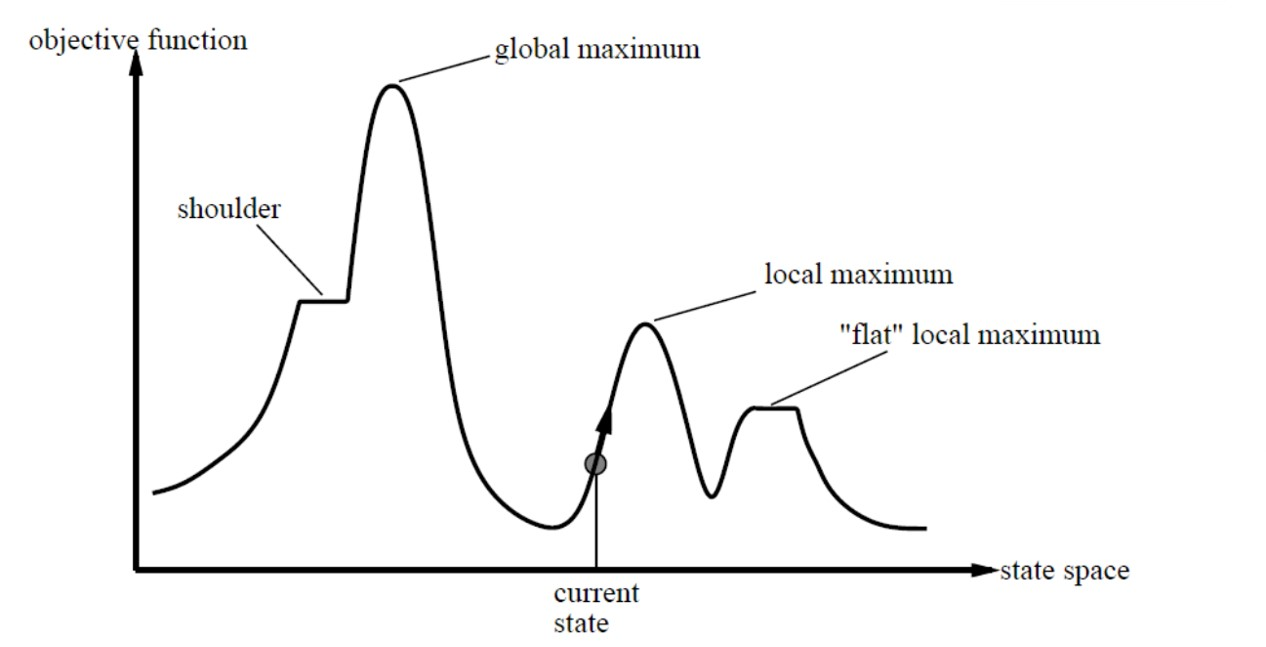
\includegraphics[width=0.7\textwidth]{immagini/spazio_stati.jpg}
	\caption*{\textit{f euristica di costo della funzione obiettivo (non del cammino)}}
\end{figure}

Uno stato ha una posizione sulla superficie e una altezza che corrisponde al valore della funzione di valutazione (funzione obiettivo).\
Un passo di un algoritmo provoca movimento sulla superficie.\

Trovare l'avvallamento più basso (e.g.\ min costo) o il picco più alto (e.g.\ max di un obiettivo).

\subsection{Ricerca in salita (Hill climbing) steepest ascent{\slash}descent}

Ricerca locale \textbf{\textit{greedy}}.\
Vengono generati i successori e valutati; viene scelto un nodo che migliora la valutazione dello stato attuale (non si tiene traccia degli altri [no albero di ricerca in memoria]):\
\begin{itemize}
	\item il migliore $\rightarrow$ Hill climbing a salita rapida
	\item uno a caso (tra quelli che salgono) $\rightarrow$ Hill climbing stocastico (anche dipendendo da pendenza)
	\item il primo $\rightarrow$ Hill climbing con prima scelta
\end{itemize}
Se non ci sono stati successori migliori l'algoritmo termina con fallimento.\

\subsubsection{L'algoritmo Hill climbing}
\begin{flushleft}
	\textbf{function} Hill-climbing (\textit{problema})

	\quad \textbf{returns} uno stato che è un massimo locale

	\qquad \textit{nodo-corrente} = CreaNodo(\textit{problema}.Stato-iniziale)

	\qquad \textbf{loop do}

	\qquad \quad \textit{vicino} = il successore di \textit{nodo-corrente} di valore più alto

	\qquad \quad \textbf{if} \textit{vicino}.Valore $\leq$ \textit{nodo-corrente}.Valore \textbf{then}

	\qquad \qquad \textbf{return} \textit{nodo-corrente}.Stato \textit{// interrompe la ricerca}

	\qquad \quad \textit{nodo-corrente} = \textit{vicino}

	\qquad \quad \textit{// (altrimenti, se vicino è migliore, continua)}
\end{flushleft}
\textbf{Nota}:\ si prosegue solo se il vicino (piu alto) è migliore dello stato corrente $\rightarrow$ Se tutti i vicini sono peggiori si ferma.\ Non c'è frontiera a cui ritornare, si tiene un solo stato.\

Tempo:\ numero cicli variabile in base al punto di partenza.

\subsubsection{Il problema delle 8 regine (formulazione a stato completo)}

\textit{Costo h}:\ numero di coppie di regine che si attaccano a vicenda (valore 17 nella figura sotto).\
Si cerca il minimo.
\begin{figure}[H]
	\centering
	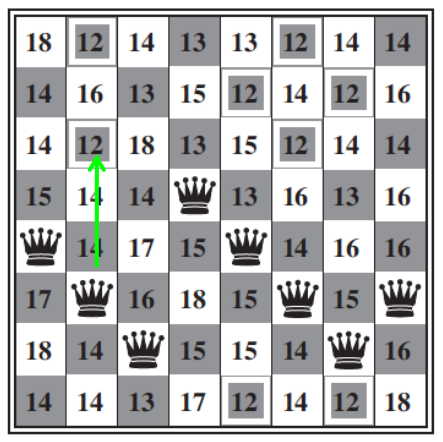
\includegraphics[width=0.4\textwidth]{immagini/otto_regine_hillClimbing.png}
\end{figure}
\noindent
I numeri sono i valori dei successori (7x8) [7 posizioni per ogni regina = su ogni colonna].\
Tra i migliori (valore 12) si sceglie a caso.\
Mininimo globale = 0.

\subsubsection{Un minimo locale}

$h = 1$
\begin{figure}[H]
	\centering
	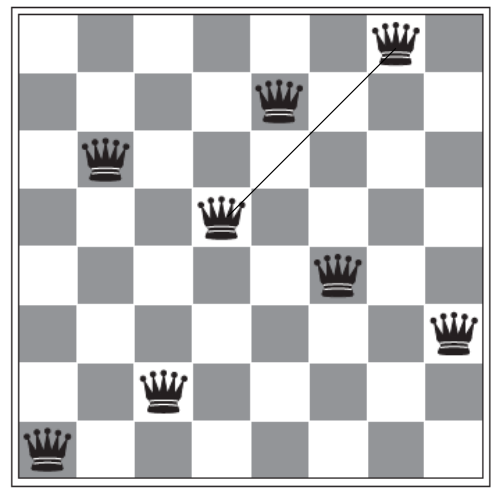
\includegraphics[width=0.4\textwidth]{immagini/minimo_locale.png}
\end{figure}

\noindent Tutti gli stati successori non migliorano la situazione (minimo locale).\
Per le 8 regine Hill climbing si blocca l'86\% delle volte, ma in media solo quattro passi per la soluzione e tre quando si blocca su $8^8 = 17$ milioni di stati.

\subsubsection{Problemi con Hill-climbing}

Se la funzione è da ottimizzare i picchi sono massimi locali o soluzioni ottimali.\

\begin{itemize}
	\item Massimi locali
	\item Pianori o spalle
	\item Crinali (o creste)
\end{itemize}

\subsubsection{Miglioramenti}
Consentire un numero limitato di mosse laterali (ossia ci si ferma per $<$ nell'algoritmo invece che per $\leq$).\
L'algoritmo sulle 8 regine ha successo nel 94\%, ma impiega in media 21 passi.\

\textbf{Hill-climbing stocastico}:\ si sceglie a caso tra le mosse in salita (magari tenendo conto della pendenza).\
Converge più lentamente ma a volte trova soluzioni migliori.\

\textbf{Hill-climbing con prima scelta}:\ può generare le mosse a caso, una alla volta, fino a trovarne una migliore dello stato corrente (si prende il primo migliore).\
Come la stocastica ma utile quando i successori sono molti (e.g.\ migliaia).

\textbf{Hill-Climbing con riavvio casuale} (\textbf{random restart}):\ ripartire da un punto scelto a caso.\
Se la probabilità di successo è \textit{p} saranno necessarie in media $1/p$ ripartenze per trovare la soluzione; per esempio 8 regine, $p=0.14$, 7 iterazioni:\ 6 fail, un successo.\
Hill-climbing con random-restart è tendenzialmente completo, insistendo si generano tutte!\
Per le regine:\ caso con 3 milioni di regine in meno di un minuto!\
Se funziona o no dipende molto dalla forma del panorama degli stati.\

\subsection{Tempra simulata}

L'algoritmo di \textbf{tempra simulata} (\textit{Simulated annealing}) [Kirkpatrick, Gelatt, Vecchi 1983] combina hill-climbing con una scelta stocastica (ma non del tutto casuale, perché poco efficiente\dots).\
Analogia con il processo di tempra dei metalli in metallurgia:\ i metalli vengono portati a temperature molto elevate (alta energia/stocasticità iniziale) e raffreddati gradualmente consentendo di cristallizzare in uno stato a (più) bassa energia.\

\noindent Ad ogni passo si sceglie un successore $n'$ a caso:
\begin{itemize}
	\item se migliora lo stato corrente viene espanso,
	\item altrimenti (caso in cui $\Delta E=f(n')-f(n) < 0$) quel nodo viene scelto con probabilità $p=e^{\Delta E/T}\ [0 \leq p \leq 1]$.
\end{itemize}
Si genera un numero casuale tra 0 e 1:\ se questo è $< p$ il successore viene scelto, altrimenti no.\
Ossia:\ \textit{p} è inversamente proporzionale al peggioramento; infatti se la mossa peggiora molto, $\Delta E$ alto negativo, la \textit{p} si abbassa.

T (temperatura) decresce col progredire dell'algoritmo (quindi anche \textit{p}) secondo un piano definito.\
Col progredire rende improbabili le mosse peggiorative.

\subsubsection{Tempra simulata:\ analisi}
La probabilità di una mossa in discesa diminuisce col tempo e l'algoritmo si comporta sempre di più come Hill Climbing.\
Se T viene decrementato abbastanza lentamente con probalità tendente ad 1 si raggiunge la soluzione ottimale.\
Analogia col processo di tempra dei metalli:
\begin{itemize}
	\item T corrisponde alla temperatura
	\item $\Delta E$ alla variazione di energia
\end{itemize}

\subsubsection{Tempra simulata:\ parametri}
Valore iniziale e decremento di T sono
parametri.\
Valori per T determinati sperimentalmente:\ il
valore \textit{iniziale} di T è tale che per valori medi di $\Delta E$, $p=e^{\Delta E/T}$ sia all'incirca 0.5.\

\subsection{Ricerca local beam}

La versione locale della \textit{beam search}.\
Si tengono in memoria \textbf{\textit{k}} stati, anziché uno solo, e ad ogni passo si generano i successori di tutti i \textit{k} stati.\
Se si trova un goal ci si ferma, altrimenti si prosegue con i \textit{k} migliori tra questi.\

\noindent \textbf{Note}:
\begin{itemize}
	\item diverso da K restart (che riparte da zero)
	\item diverso da beam search: perché?
	\item $k=1$ o illimitato a cosa portano?
\end{itemize}

\subsection{Beam search stocastica}

Si introduce un elemento di casualità come in un processo di \textbf{selezione naturale} (diversificare la nuova generazione).\
Nella variante stocastica della \textit{local beam}, si scelgono \textit{k} successori, ma con probabilità maggiore per i migliori.\
La terminologia:
\begin{itemize}
	\item \textit{organismo} [stato]
	\item \textit{progenie} [successori]
	\item \textit{fitness} [il valore della f], idoneità
\end{itemize}

\subsubsection{Algoritmi genetici}
Sono \textbf{varianti} della \textbf{beam search stocastica} in cui gli stati successori sono ottenuti combinando due stati genitore (anziché per evoluzione).\
La terminologia:\
\begin{itemize}
	\item \textbf{popolazione} di \textbf{individui} [stati]
	\item \textbf{fitness}
	\item \textbf{accoppiamenti} + \textbf{mutazione genetica}
	\item \textbf{generazioni}
\end{itemize}
\textbf{Popolazione} iniziale:\ \textit{k} stati/\textbf{individui} generati casualmente e ogni individuo è rappresentato come una stringa.
Gli individui sono valutati da una \textbf{funzione di fitness}.\

\noindent Si \textbf{selezionano} gli individui per gli ``\textbf{accoppiamenti}'' con una probabilità proporzionale alla fitness.\
Le coppie danno vita alla generazione successiva combinando materiale genetico (crossover) e con un meccanismo aggiuntivo di mutazione genetica (casuale), la popolazione ottenuta dovrebbe essere migliore.\
La cosa si ripete fino ad ottenere stati abbastanza buoni (stati obiettivo).

\begin{figure}[H]
	\centering
	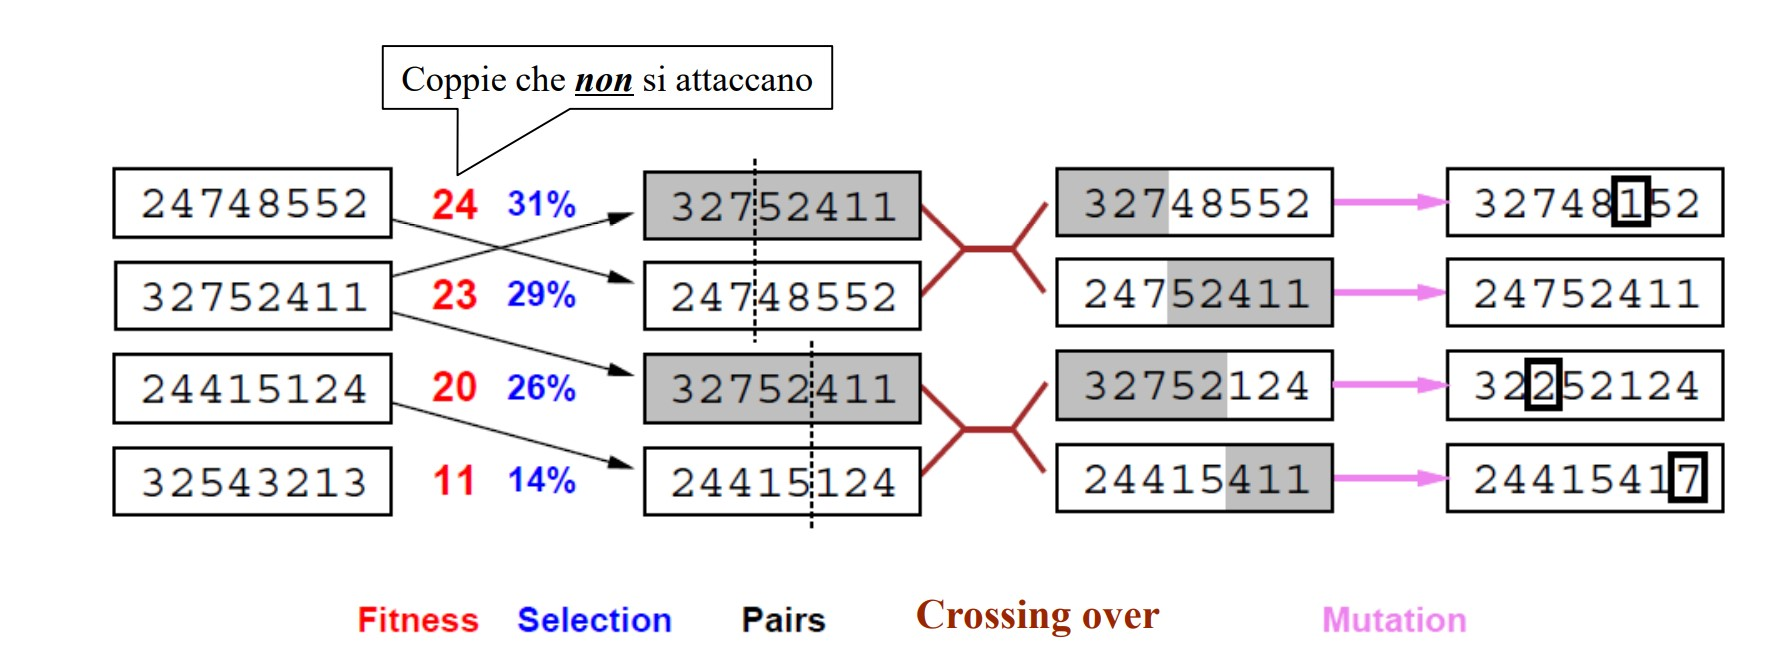
\includegraphics[width=\textwidth]{immagini/Alg_genetici.jpg}
\end{figure}

\noindent Per ogni coppia viene scelto un punto di \textbf{\textit{crossing over}} e vengono generati due figli scambiandosi pezzi (del DNA).\
Viene infine effettuata una \textit{mutazione} casuale che dà luogo alla prossima generazione.\

\begin{figure}[H]
	\centering
	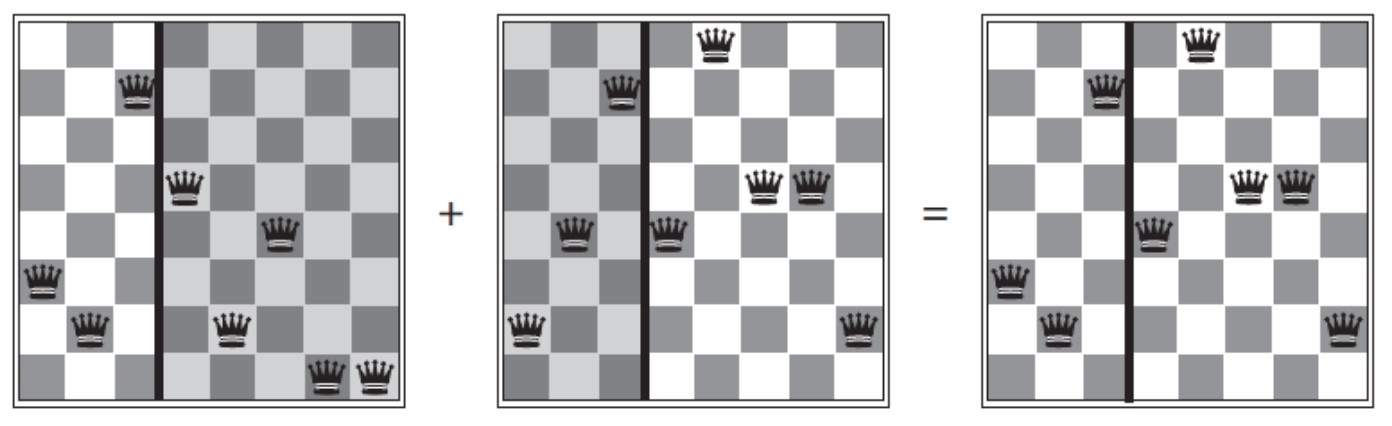
\includegraphics[width=0.8\textwidth]{immagini/8regine_gen.jpg}
	\caption*{\footnotesize Le parti chiare sono passate al figlio, le parti grigie si perdono.\

		Se i genitori sono molto diversi anche i nuovi stati sono diversi.\
		All'inizio spostamenti maggiori che poi si raffinano.}
\end{figure}

\noindent Suggestivi (area del \textit{Natural computing}:\ e.g.\ swarm,\ \dots).\
Usati in molti problemi reali e.g.\ configurazione di circuiti e scheduling di lavori.\
Combinano la tendenza a salire della beam search stocastica e l'interscambio di informazioni tra thread paralleli di ricerca (blocchi utili che si combinano).\

Funziona meglio se il problema (soluzioni) ha componenti significative rappresentate in sottostringhe $\rightarrow$ \textbf{punto critico}:\ la rappresentazione del problema in stringhe.

\section{Spazi continui}

Molti casi reali hanno spazi di ricerca continua, e.g.\ fondamentale per Machine Learning!\

Stato descritto da variabili continue, $x_1,\ \dots,\ x_n$, vettore \textbf{\textit{x}}.\
Prendiamo ad esempio movimenti in spazio 3D, con posizione data da $x=(x_1,\ x_2,\ x_3)$.\

Apparentemente ostico, fattori di ramificazione infiniti con gli approcci precedenti.\
In realtà ci sono molti strumenti matematici per spazi continui, che portano ad approcci anche molto efficienti\dots

\subsubsection{Gradient}

Se la \textit{f} è continua e differenziabile, e.g.\ quadratica rispetto ad \textbf{\textit{x}} (vettore).\
Il minimo o massimo si può cercare utilizzando il gradiente, che restituisce la direzione di massima pendenza nel punto.\

\noindent Data \textit{f} obiettivo
\[
	\nabla f = \left( \frac{\partial f}{\partial x_1},\ \frac{\partial f}{\partial x_2},\ \frac{\partial f}{\partial x_3} \right)
\]
Hill climbing iterativo:
\[
	x_{new} = x + \eta\nabla f\left(x\right)
\]
Quantifica lo spostamento, senza cercarlo tra gli infiniti possibili successori!\

Uso + per salire (maximization).

Uso – per scendere (minimization).

$\eta$ (eta):\ step size.

\begin{figure}[H]
	\centering
	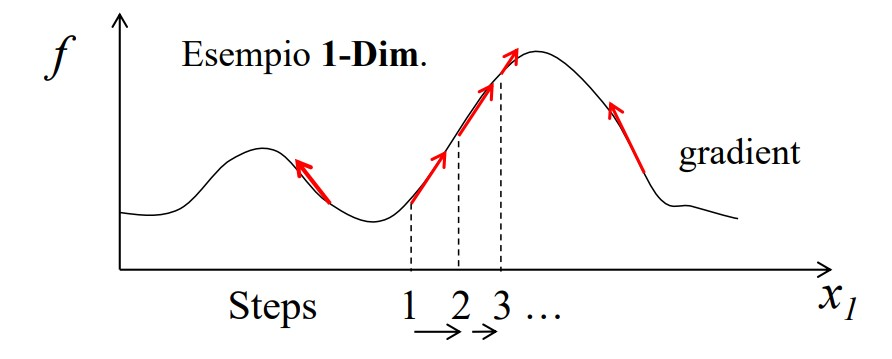
\includegraphics[width=0.6\textwidth]{immagini/Gradient.jpg}
	\caption*{Spostamenti guidati dal gradiente}
\end{figure}

\noindent \textbf{Nota generale}:\ non sempre è necessario il min/max assoluto.

\section{Assunzioni sull'ambiente da riconsiderare}

\subsubsection{Ambienti più realistici}
Gli agenti \textit{risolutori di problemi} ``classici'' assumono:
\begin{itemize}
	\item ambienti completamente osservabili;
	\item azioni/ambienti deterministici;
	\item il piano generato è una sequenza di azioni che può essere generato \textit{offline} e eseguito senza imprevisti;
	\item le percezioni non servono se non nello stato iniziale.
\end{itemize}

\subsubsection{Soluzioni più complesse}
In un ambiente parzialmente osservabile e non deterministico le \textbf{percezioni} sono importanti perché
restringono gli stati possibili e informano sull'effetto dell'azione.\
Più che un piano l'agente può elaborare una ``\textit{strategia}'', che tiene conto delle diverse eventualità:\ un \textbf{piano con contigenza}.

\subsection{Azioni non deterministiche}

\subsubsection{L'aspirapolvere imprevedibile}

Comportamento:\ se aspira in una stanza sporca la pulisce, ma talvolta pulisce anche una stanza adiacente; se aspira in una stanza pulita, a volte rilascia sporco.\

Variazioni necessarie al modello:
\begin{itemize}
	\item Il modello di transizione restituisce un insieme di stati:\ l'agente non sa in quale si troverà.
	\item Il piano di contingenza sarà un piano condizionale e magari con cicli.
\end{itemize}

\begin{figure}[H]
	\centering
	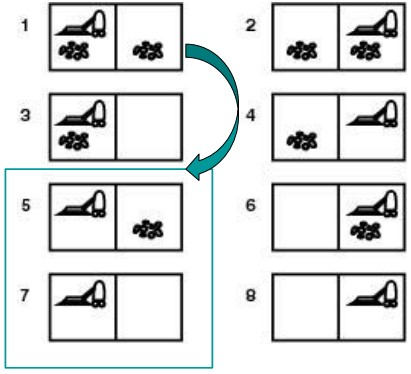
\includegraphics[width=0.4\textwidth]{immagini/nDeterm.jpg}
\end{figure}
\noindent Esempio:\ \textit{Risultati}(Aspira, 1) = \{5, 7\}

\noindent Piano possibile

\begin{verbatim}
[Aspira,
    if stato=5
	then [Destra, Aspira]
    else [ ]
    ]
\end{verbatim}

\subsubsection{Come si pianifica:\ alberi di ricerca AND-OR}

Nodi OR le scelte dell'agente (1 sola azione).\
Nodi AND le diverse contingenze (le scelte dell'ambiente, piu stati possibili), da considerare tutte.\

Una soluzione a un problema di ricerca AND-OR è un \textbf{albero} che ha un nodo obiettivo in ogni foglia:\ specifica un'unica azione nei nodi OR e include tutti gli archi uscenti da nodi AND (tutte le contingenze).

\begin{figure}[H]
	\centering
	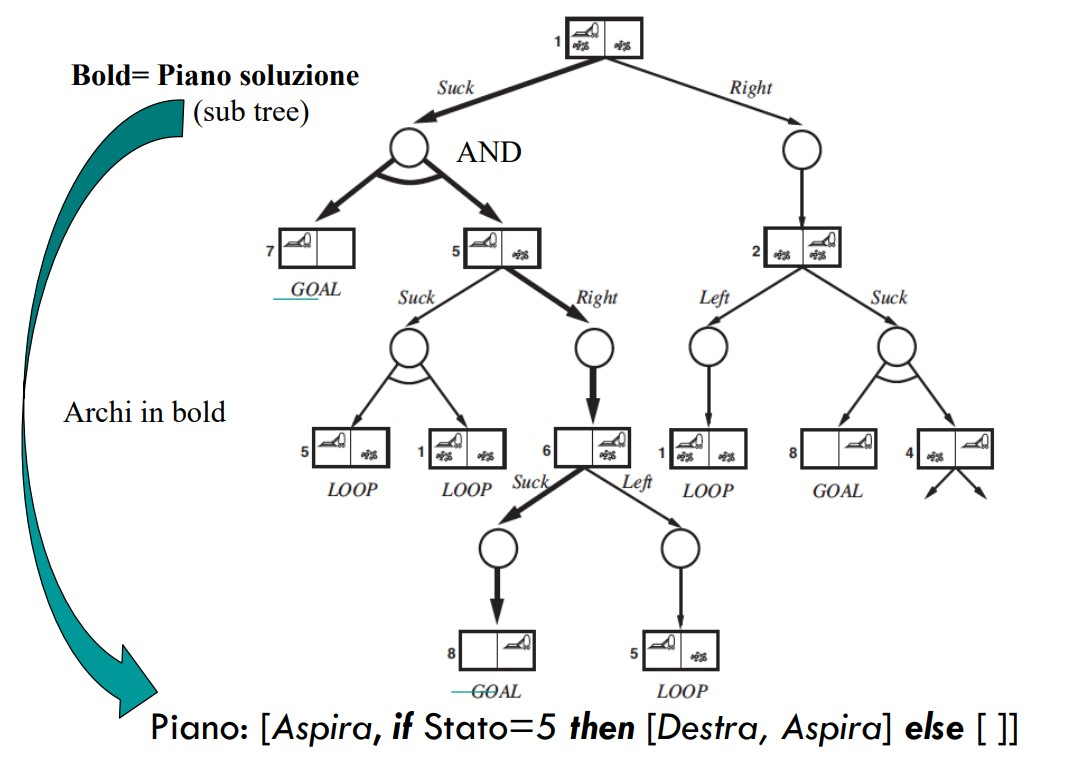
\includegraphics[width=0.7\textwidth]{immagini/AND-OR.jpg}
\end{figure}
